\RequirePackage[l2tabu,orthodox]{nag}

% TODO: decide if one-sided/two-sided
%\documentclass[headsepline,footsepline,footinclude=false,fontsize=11pt,paper=a4,listof=totoc,bibliography=totoc,BCOR=12mm,DIV=12]{scrbook} % two-sided
\documentclass[headsepline,footsepline,footinclude=false,oneside,fontsize=11pt,paper=a4,listof=totoc,bibliography=totoc]{scrbook} % one-sided



\PassOptionsToPackage{table,svgnames,dvipsnames}{xcolor}

\usepackage[utf8]{inputenc}
\usepackage[T1]{fontenc}
\usepackage[sc]{mathpazo}
\usepackage[american]{babel}
\usepackage[autostyle]{csquotes}
\usepackage[%
  backend=biber,
  url=false,
  style=alphabetic,
  maxnames=4,
  minnames=3,
  maxbibnames=99,
  firstinits,
  uniquename=init]{biblatex} % TODO: adapt bibliography style
\usepackage{graphicx}
\usepackage{scrhack} % necessary for listings package
\usepackage{listings}
\usepackage{lstautogobble}
\usepackage{tikz}
\usepackage{pgfplots}
\usepackage{pgfplotstable}
\usepackage{booktabs}
\usepackage[final]{microtype}
\usepackage{caption}
\usepackage{graphicx}
\usepackage{gensymb}
\usepackage[hidelinks]{hyperref} % hidelinks removes colored boxes around references and links
\usepackage[toc,nonumberlist,acronym]{glossaries} % TODO: remove if glossary not needed
\usepackage{textcomp} 
\usepackage{hyperref}
\usepackage{color}
\hypersetup{
      % links in new PDF window
   colorlinks=false,       % false: boxed links; true: colored links
   linkcolor=blue}

\bibliography{bibliography/literature}{}

\setkomafont{disposition}{\normalfont\bfseries} % use serif font for headings
\linespread{1.05} % adjust line spread for mathpazo font

% Settings for glossaries TODO: remove the following block if glossary not needed
\renewcommand{\glsnamefont}[1]{\normalfont\bfseries #1} % use serif font for glossary entry titles
\makeglossaries{}

% Settings for pgfplots
\pgfplotsset{compat=1.9} % TODO: adjust to your installed version
\pgfplotsset{
  % For available color names, see http://www.latextemplates.com/svgnames-colors
  cycle list={CornflowerBlue\\Dandelion\\ForestGreen\\BrickRed\\},
}

% Settings for lstlistings
\lstset{%
  basicstyle=\ttfamily,
  columns=fullflexible,
  autogobble,
  keywordstyle=\bfseries\color{MediumBlue},
  stringstyle=\color{DarkGreen}
  }

% Commands to be used within the TUM report document
% Included by MAIN.TEX
% Please include your own cool commands here. 
% Be only sure to comment it sufficiently so others can use it.

%-------------------------------------------------------------
%                      Own Commands
%-------------------------------------------------------------
\DeclareMathOperator*{\st}{\text{ s.t. }}
\DeclareMathOperator*{\rev}{rev}
\DeclareMathOperator*{\enc}{enc}
\DeclareMathOperator*{\argmin}{argmin}
\DeclareMathOperator*{\argmax}{argmax}

\DeclareMathOperator*{\prerank}{pre-rank}
\DeclareMathOperator*{\postrank}{post-rank}

\DeclareMathOperator*{\preselect}{pre-select}
\DeclareMathOperator*{\postselect}{post-select}

\DeclareMathOperator*{\firstchild}{first-child}
\DeclareMathOperator*{\lastchild}{last-child}
 
\DeclareMathOperator*{\nextsibling}{next-sibling}
\DeclareMathOperator*{\prevsibling}{prev-sibling}

\DeclareMathOperator*{\nextsiblingk}{next-sibling^{k-1}}
\DeclareMathOperator*{\prevsiblingk}{prev-sibling^{k-1}}
\DeclareMathOperator*{\enclosek}{enclose^{d}}

\DeclareMathOperator*{\subtreesize}{subtree-size}

\DeclareMathOperator*{\fwdsearch}{fwd-search}
\DeclareMathOperator*{\bwdsearch}{bwd-search}

\DeclareMathOperator*{\parent}{parent}
\DeclareMathOperator*{\enclose}{enclose}
\DeclareMathOperator*{\rmqi}{rmqi}
\DeclareMathOperator*{\rmq}{rmq}
\DeclareMathOperator*{\RMQ}{RMQ}
\DeclareMathOperator*{\RMQi}{RMQi}
\DeclareMathOperator*{\findopen}{findopen}
\DeclareMathOperator*{\findclose}{findclose}
\DeclareMathOperator*{\inspect}{inspect}
\DeclareMathOperator*{\isleaf}{isleaf}
\DeclareMathOperator*{\isancestor}{isancestor}
\DeclareMathOperator*{\depth}{depth}
\DeclareMathOperator*{\levelnext}{level-next}
\DeclareMathOperator*{\levelprev}{level-prev}
\DeclareMathOperator*{\levellmost}{level-lmost}
\DeclareMathOperator*{\levelrmost}{level-rmost}
\DeclareMathOperator*{\deepestnode}{deepest-node}
\DeclareMathOperator*{\levelancestor}{level-ancestor}
\DeclareMathOperator*{\lca}{lca}
\DeclareMathOperator*{\ssum}{sum}
\DeclareMathOperator*{\childselectfromleft}{left-select-child}
\DeclareMathOperator*{\childselectfromright}{right-select-child}

\DeclareMathOperator*{\rankopen}{rank_1}
\DeclareMathOperator*{\rankclose}{rank_0}

\DeclareMathOperator*{\selectopen}{select_1}
\DeclareMathOperator*{\selectclose}{select_0}

\DeclareMathOperator*{\selectopenfrom}{selectfrom_1}
\DeclareMathOperator*{\selectclosefrom}{selectfrom_0}

\DeclareMathOperator*{\excess}{pi}
\DeclareMathOperator*{\opencounter}{phi}
\DeclareMathOperator*{\closecounter}{psi} 

%-------------------------------------------------------------
% math stuff -------------------------------------------------

% nice R, N, C
\newcommand{\nat}{\mathbb{N}}
\newcommand{\real}{\mathbb{R}}
\newcommand{\compl}{\mathbb{C}}

% norm
\newcommand{\norm}[1]{\left\| #1 \right\|}

% un demi
\newcommand{\half}{\frac{1}{2}}

% parantheses
\newcommand{\parenth}[1]{ \left( #1 \right) }
\newcommand{\bracket}[1]{ \left[ #1 \right] }
\newcommand{\accolade}[1]{ \left\{ #1 \right\} }
%\newcommand{\angle}[1]{ \left\langle  #1 \right\rangle }

% partial derivative: %#1 function, #2 which variable
% simple / single line version
\newcommand{\pardevS}[2]{ \delta_{#1} f(#2) }
% fraction version
\newcommand{\pardevF}[2]{ \frac{\partial #1}{\partial #2} }

% render vectors: 3 and 4 dimensional
\newcommand{\veciii}[3]{\left[ \begin{array}[h]{c} #1 \\ #2 \\ #3	\end{array} \right]}
\newcommand{\veciv}[4]{\left[ \begin{array}[h]{c} #1 \\ #2 \\ #3 \\ #4	\end{array} \right]}

% render matrices: 3  dimensional (arguments in row first order)
\newcommand{\matiii}[9]{\left[ \begin{array}[h]{ccc} #1 & #2 & #3 \\ #4 & #5 & #6 \\ #7 & #8 & #9	\end{array} \right]}
%DOESN'T WORK,DON'T KNOW WHY \newcommand{\mativ}[16]{\left[ \begin{array}[h]{cccc} #1 & #2 & #3 & #4 \\ #5 & #6 & #7 & #8 \\ #9 & #10 & #11 & #12 \\ #13 & #14 & #15 & #16 \end{array} \right]}


%-------------------------------------------------------------
%-------------------------------------------------------------


%-------------------------------------------------------------
% some abreviations ------------------------------------------
\newcommand{\Reg}{$^{\textregistered}$}
\newcommand{\reg}{$^{\textregistered}$ }
\newcommand{\Tm}{\texttrademark}
\newcommand{\tm}{\texttrademark~}
\newcommand {\bsl} {$\backslash$}

%-------------------------------------------------------------
%-------------------------------------------------------------


%-------------------------------------------------------------
% formating --------------------------------------------------

% Theorem & Co environments and counters
\newtheorem{theorem}{Theorem}[chapter]
\newtheorem{lemma}[theorem]{Lemma}
\newtheorem{corollary}[theorem]{Corollary}
\newtheorem{remark}[theorem]{Remark}
\newtheorem{definition}[theorem]{Definition}
\newtheorem{equat}[theorem]{Equation}
\newtheorem{example}[theorem]{Example}
%\newtheorem{algorithm}[theorem]{Algorithm}

% inserting figures
\newcommand{\insertfigure}[4]{ % Filename, Caption, Label, Width percent of textwidth
	\begin{figure}[htbp]
		\begin{center}
			\includegraphics[width=#4\textwidth]{#1}
		\end{center}
		\vspace{-0.4cm}
		\caption{#2}
		\label{#3}
	\end{figure}
}




% referecing figures

\newcommand{\refFigure}[1]{ %label
	figure \ref{#1}
}
\newcommand{\refChapter}[1]{ %label
	chapter \ref{#1}
}

\newcommand{\refSection}[1]{ %label
	section \ref{#1}
}

\newcommand{\refParagraph}[1]{ %label
	paragraph \ref{#1}
}

\newcommand{\refEquation}[1]{ %label
	equation \ref{#1}
}

\newcommand{\refTable}[1]{ %label
	table \ref{#1}
}




\newcommand{\rigidTransform}[2]
{
	${}^{#2}\!\mathbf{H}_{#1}$
}

%code, in typewriter
\newcommand{\code}[1]
 {\texttt{#1}}

% comment that appears on the border - very practical !!!
\newcommand{\comment}[1]{\marginpar{\raggedright \noindent \footnotesize {\sl #1} }}

% page clearing
\newcommand{\clearemptydoublepage}{%
  \ifthenelse{\boolean{@twoside}}{\newpage{\pagestyle{empty}\cleardoublepage}}%
  {\clearpage}}


%-------------------------------------------------------------
%-------------------------------------------------------------


\newcommand{\etAl}{\emph{et al.}\mbox{ }}


% TODO: remove if glossary not needed
%\newglossaryentry{computer}
{
  name=computer,
  description={is a machine that\ldots}
}

%\chapter*{Acronyms}

\begin{acronym}[EDF]
	\acro{ECU}{Electronic Control Unit}
	\acro{IPC}{Inter Process Communication}
	\acro{ITS}{Intelligent Transportation System}
	\acro{KIA4SM}{Cooperative Integration Architecture for Future Smart Mobility Solutions}
	\acro{EDF}{Earliest Deadline First}
	\acro{FP}{Fixed Priority}
	\acro{IPC}{Inter-Process Communication}
	\acro{SMP}{Symmetric Multi Processing}
	\acro{RPC}{Remote Procedure Calls}
	\acro{OC}{Organic Computing}
	\acro{OC}{Object Capability System}
	\acro{PD}{Protection Domain}
	\acro{API}{Application Programming Interface}
	\acro{RCU}{Read Copy Update}
	\acro{STM}{Software Transactional Memory}
	\acro{CPU}{Central Processing Unit}
	\acro{OS}{Operating System}
	\acro{L4Re}{L4 Runtime Environment}
	\acro{QEMU}{Quick Emulator}
	\acro{RAM}{Random Access Memory}
	\acro{RM} {Region Manager}
	\acro{RQ}{Ready Queue}
	\acro{UTCB} {User-level Thread Control Block}
	\acro{GNU}{GNU's Not Unix}
	\acro{GCC}{GNU Compiler Collection}
	\acro{GMBH}{full name}
	\acro{GPL}{full name}
\end{acronym}

\begin{document}

%\begin{titlepage}
  % HACK for two-sided documents: ignore binding correction for cover page.
  % Adapted from Markus Kohm's KOMA-Script titlepage=firstiscover handling.
  % See http://mirrors.ctan.org/macros/latex/contrib/koma-script/scrkernel-title.dtx,
  % \maketitle macro.
  \oddsidemargin=\evensidemargin\relax
  \textwidth=\dimexpr\paperwidth-2\evensidemargin-2in\relax
  \hsize=\textwidth\relax

  \centering

  \vspace{40mm}
  
\includegraphics[width=40mm]{logos/tum}

  \vspace{5mm}
  {\huge\MakeUppercase{\getFaculty{}}}\\

  \vspace{5mm}
  {\large\MakeUppercase{\getUniversity{}}}\\

  \vspace{20mm}
  {\Large \getDoctype{}}

  \vspace{15mm}
  {\huge\bfseries \getTitle{}}

  \vspace{15mm}
  {\LARGE \getAuthor{}}

  \vspace{20mm}
  
\includegraphics[width=20mm]{logos/faculty}
\end{titlepage}


\frontmatter{}

\begin{titlepage}
  \centering

  \IfFileExists{logos/tum.pdf}{%
    \includegraphics[height=20mm]{logos/TUMLogo.pdf}
  }{%
    \vspace*{10mm}
  }

  \vspace{5mm}
  {\huge\MakeUppercase{\getFaculty{}}}\\

  \vspace{5mm}
  {\large\MakeUppercase{\getUniversity{}}}\\

  \vspace{10mm}
  {\Large \getDoctype{}}

  \vspace{10mm}
  {\LARGE\bfseries \getTitle{}}

  \vspace{10mm}
  {\LARGE\bfseries \getTitleGer{}}

  \vspace{10mm}
  \begin{tabular}{l l}
    Author: & \getAuthor{} \\
    Supervisor: & \getSupervisor{} \\
    Advisor: & \getAdvisor{} \\
    Submission Date: & \getSubmissionDate{} \\
  \end{tabular}

  \IfFileExists{logos/faculty.pdf}{%
    \vfill{}
    
\includegraphics[height=20mm]{logos/faculty.pdf}
  }{}
\end{titlepage}
%\thispagestyle{empty}
\vspace*{0.8\textheight}
\noindent
I confirm that this \MakeLowercase{\getDoctype{}} is my own work and I have documented all sources and material used.

\vspace{15mm}
\noindent
\getSubmissionLocation{}, \getSubmissionDate{} \hspace{5cm} \getAuthor{}

\cleardoublepage{}

%\addcontentsline{toc}{chapter}{Acknowledgments}
\thispagestyle{empty}

\vspace*{20mm}

\begin{center}
{\usekomafont{section} Acknowledgments}
\end{center}

\vspace{10mm}

%TODO: Acknowledgments

%Writing this master's thesis would not have been possible without the help of these people. 
%First, I would like to thank my advisors Daniel Krefft and Sebastian Ekcl, who immediately accepted my request to do masters thesis and guided me to chose the projects. Special thanks to Daniel Krefft for his brilliant advices which he has given me every time we had a discussion.
%
%Thanks to Prof.Baumgarten for allowing me to do my research and for providing all the facilities at the chair. 
%
%Thanks to Paul Nieleck, who is finished his master thesis at the department for excellent collaboration and sharing his knowledge on the project. 
%
%Thanks to Alexander Reisner who is working at the department, for sharing his timely invaluable experience on the project. 
%
%%Thanks to Madhura Kumaraswamy for her help during my thesis. 
%
%Thank you to my family for providing me the freedom and support that required me to come to Germany for doing my masters. 


\cleardoublepage{}

%\chapter{\abstractname}

%TODO: Abstract

%Motivation/Problem statement Aims and objectives

This thesis introduces a method for updating the task ready queues in the Genode Operating System Framework and the L4/Fiasco.OC microkernel. The presented method will be used in Organic Computing paradigm's Observer-Controller architecture. The Observer monitors the system and gathers the data and passes it to the Controller, which processes the data and takes a decision to schedule the tasks. This requires a method in place to provide the synchronized access to ready queue and update the tasks.

%What does the thesis do?
%The limitations in accessing the kernel ready queue from a high-level component led to the development of a split module. Accordingly,
The implementation of the ready queue update mechanism consists of a high-level Genode component and a low-level kernel module. The Genode component communicates with the Controller via a shared dataspace and receives the tasks to be updated and then passes them to the kernel module. The kernel module identifies the corresponding kernel threads and updates them to the ready queue. Various synchronization methods are presented in this thesis with special importance to lock-free algorithms. RCU and STM synchronization methods are suggested for synchronizing the kernel ready queue access. 

%Findings and conclusions
Tests of the task-ready queue update mechanism showed that the threads can be updated successfully to the ready queue and executed. On the other hand, complete ready queue swapping leaves the system in an unstable state. The high-level component is able to communicate successfully with the Controller via Genode's shared dataspace. The proposed design and implementation can be successfully used in the Observer-Controller architecture and it serves as a good starting point for the KIA4SM project's goal of having the ready queue update mechanism as a fully high-level component.

%vision of providing a homogeneous execution environment for heterogeneous hardware systems involves in using universally applicable ECUs and having flexible task scheduling on ECUs. This requires having a intelligent system in place to take decisions, which is solved by Organic-Computing paradigm's Observer-Controller architecture, which has an Observer that monitors the system and gathers the data and pass it to the Controller, which processes the data and takes a decision to schedule the tasks. This requires a method in place to provide the synchronized access to ready queue and update the tasks.
\microtypesetup{protrusion=false}
\tableofcontents{}
\microtypesetup{protrusion=true}

\mainmatter{}


\chapter{Introduction}\label{chapter:introduction}

Network on Chip (NoC) is a communication subsystem on an integrated circuit typically between intellectual property(IP) cores in a System on Chip(SoC). In the modern NoCs there are numerous possible topologies and similarly in the integration of IPs for SoCs there can a lot of possible architectures. 

In order to find the optimal solution, some algorithms model the system as a graph and then optimize it iteratively. Graph algorithms play an important role in the these optimizations in particular graph transformation or graph rewriting techniques.

Graph transformation concerns the technique of creating a new graph out of an original graph algorithmically. The basic idea is that the,
design is represented as graph and the transformations are carried out based on transformation rules. Such rules consist of an original graph,
a subgraph which is to be matched on to the original graph and a replacing graph, which will replace the matched subgraph. 
Formally, a graph rewriting system usually consists of a set of graph rewrite rules of the form $L -> R$, with $L$ being called the pattern graph (or left-hand side, LHS) and $R$ being called the replacement graph (or right hand-side of the rule, RHS). A graph rewrite rule is applied on the host graph by searching for an occurrence of the pattern graph and by replacing the found occurrence by an instance of the replacement graph.

As we apply these series of rules (often interchangeably), the number of resultant graphs increase significantly, which means more designs. Sometimes there can be lot duplicates
in the resultant graphs as we apply rules interchangeably. Therefore, we need to identify the potential duplicates in order to avoid unnecessary designs. Usually the rule applying process goes in layers and represents the resultant graphs as nodes of a tree. There should be a logic to identify repeated node(graph in a tree) and merge this resultant node with the existing node. This can be termed as \texttt{node merging} problem. 

\section{Tasks}
As explained before, to do node merging, so we need to identify duplicates, we need to compare graphs. Now this problem became a exact graph matching or graph isomorphism problem. This calls for a fast, efficient and reliable graph isomorphism algorithm since, each time we apply a rule we get a new graph, which has to be compared with all the previously obtained graphs. 
For example, we apply a rule and get graph $n$, which has to be compared with $n-1$ times. For n rules the number of comparisons given by \ref{compraison_number}, 
\begin{equation}
            n(n-1)/2 
        \label{compraison_number}
\end{equation}

In addition to node merging, a little work was carried out on creating a Graphical editor for changing and viewing NoCs. The NoC can be modeled using Eclipse Modeling Framework(EMF). 
Graphical Modeling Framework (GMF) is an Eclipse Modeling Project, project that aims to provide a generative bridge between the Eclipse Modeling Framework and Graphical Editing Framework. 

Chapter 2 discusses the details of node-merging such as logic, graph isomorphism problem and algorithm, results. 
Chapter 3 discusses the introduction and possibility of using GMF in the current project.
Chapter 4 gives conclusion and possible future work. 



\chapter{Node Merging} \label{nodemerging}
	This chapter explains the process of node merging and the VF2 algorithm in detail.

\section{Node Merging Implementation}
In graph transformation, rules are applied on the host graph and the resulting graphs are represented as nodes of a tree. When the application of a rule gives a new graph (node), it needs to be compared with the existing tree nodes. If that node exists already, an edge is added to that node, otherwise, a new node is created. The corresponding code listing can be seen below.

\begin{lstlisting}[language = Java,frame = single]
 for(E rule: rules){
 V newNode = ruleExecutor.execute(node, rule)
 if(newNode != null) {
 /* For all the older nodes in the tree check if it has any match*/
 for(V oldNode:tree.getVertices()){  
        if(nodeComparator.compare(oldNode, newNode)){
	            /* If yes then just add an edge to the existing node */
            Integer edgeId = new Integer(tree.getEdgeCount());
     	    edgeIdToRuleMap.put(edgeId, rule);
    	    tree.addEdge(edgeId, node, oldNode, EdgeType.DIRECTED);
            flag = true;
            break;
        }
    }
 /* If this is a unique graph, create a new node and add it to the tree*/
	   if(!flag){
		    Integer edgeId = new Integer(tree.getEdgeCount()); 
    		edgeIdToRuleMap.put(edgeId, rule);	
	    	tree.addVertex(newNode);
		    tree.addEdge(edgeId, node, newNode, EdgeType.DIRECTED);
        }
    }
}
\end{lstlisting}

\section{Graph Matching}
Two graphs are said to be isomorphic if they have the vertices connected in the same way. Formally, two graphs $G$ and $H$ with graph vertices $V_n =\{1,2,...,n\}$ are said to be isomorphic if there is a permutation $p$ of $V_n$ such that $\{u,v\}$ is in the set of graph
edges $E(G)$ iff $\{p(u),p(v)\}$ is in the set of graph edges $E(H)$ \cite{iso1}.

Exact graph matching or graph isomorphism problem is the computational problem of determining whether two finite graphs are isomorphic. The importance of Graph isomorphism algorithms is very high in multiple fields, such as electronic design automation, chemistry and molecular biology etc.

\subsection{Complexity}
Besides its practical importance, the graph isomorphism problem is a curiosity in computational complexity theory as it one of a
very small number of problems belonging to NP, neither known to be solvable in polynomial time nor NP-complete. At the same time, isomorphism
for many special classes of graphs can be solved in polynomial time and in practice, graph isomorphism can often be solved efficiently \cite{iso2}.
This is a special case of the subgraph isomorphism problem, which is known to be NP-complete. However Laszlo Babai has claimed that the 
Graph Isomorphism can be solved in quasipolynomial time. Quantities which are exponential in some power of a logarithm are called “quasipolynomial” \cite{iso3}.

\subsection{Negative checks}
Before going into the algorithm, negative checks can be performed to avoid the graph matching algorithm and yield faster results.
\begin{enumerate}
\item \texttt{Vertex number equivalence:} The number of vertices should be equal

\item \texttt{Edge Count equivalence:} The sum of the edges should be equal

\item \texttt{Edge order check:} This is one of the important checks because when the graphs don't change much, the edge and vertices numbers may not change. Therefore, sorting the edge arrays and comparing them will give good candidates for the matching algorithm.
\end{enumerate}

\section{VF2 Algorithm}
Algorithms such as Ullman, NAUTY and VF2 can be used to solve the graph isomorphism problem. The VF2 algorithm is one of the fastest algorithms for graphs containing many vertices. The software VFLib and the VF2 algorithm are good starting points for writing the custom implementation. 

The VFLib defines a single interface (state) that a variety of subgraph isomorphism matchers can implement in order for it to work interchangeably. The challenges faced during this implementation  were firstly, to understand the intricate VF2 algorithm and secondly, customizing the algorithm to the current problem. One of the ways to understand any graph matching algorithm is to understand the commonalities among all of the approaches currently used . 

A note on the terminology: In graph comparison one graph will be compared to another, can be denoted as graph1 and graph2 or source graph and target graph. 

The commonalities among all graph matching algorithms are:\cite{ric}
\begin{itemize}
\item \texttt{Recursion:} Any implementation typically has a method that calls itself

\item\texttt{State accumulation:} The recursive method gradually builds up a map of nodes from source graph to target graph, one pair of nodes at a time. Sometime it fails, so it needs to go back to last successful match (backtrack). When it succeeds and needs to report success.

\item \texttt{Mapping:} The implementation typically uses an internal map to keep track of what it's done. So getting mapped nodes is easy.
\end{itemize}
 
\begin{figure}
\centerline{
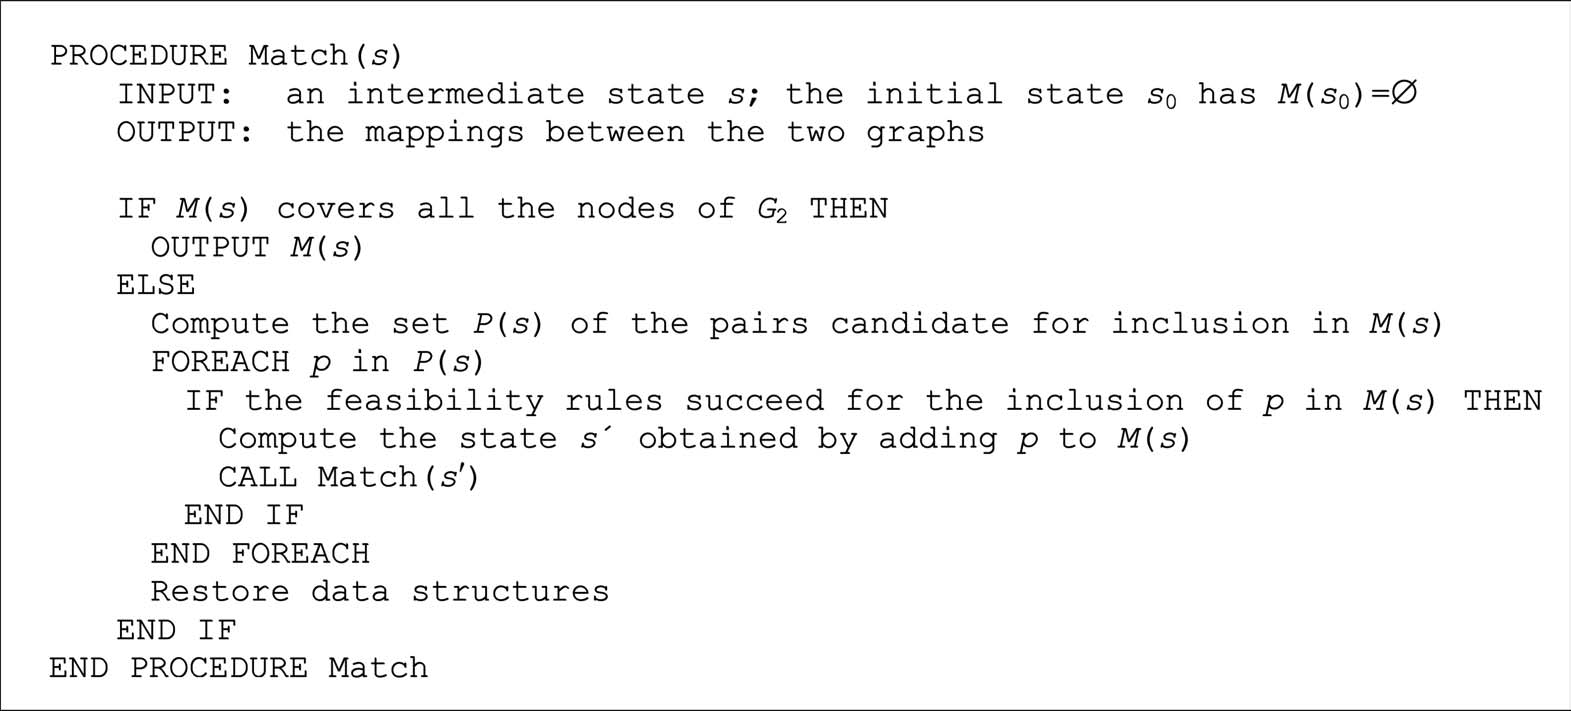
\includegraphics[width=1.0\columnwidth]{figures/vf2_image.png}
}
\caption{VF2 algorithm }
\label{vf2}
\end{figure}

The basic idea behind the VF2 algorithm is that it tries to find the mapping of vertices between two graphs. 
This process of finding the mapping function can be suitably
described by \textit{State Space Representation (SSR)} \cite{vf2}.
Each state $s$ of the matching process can be associated to a partial mapping solution $M(s)$, which contains only subset of the complete mapping. A transition from a generic states to a successor state $s'$, represents the addition of a pair of matched nodes to partial mapping associated to s in the SSR. The algorithm explores the search graph in the SSR according to a depth-first search strategy. 

In figure \ref{vf2}, the Match(s) procedure plays the role of recursive function, while $s$ and $s'$ play the dual role of state accumulators and feature comparators. $P(s)$ represents the set of candidates to be added to state $s$. A set of feasibility rules can be defined to check the consistency condition. These rules can be both syntactic(depend only on the structure of the graph) and semantic (depend on the attributes of nodes and edges).

\subsection{Tracing of VF2 algorithm}

This section explains the tracing process of the VF2 algorithm. Consider two simple graphs $g1$ and $g2$ (Figure \ref{tikz1}) and assume that node $1$ is equivalent to $a$, $2$ is equivalent to $b$ and so on, both semantically and syntactically (color property). We have a candidate list (all possible mappings) and a $map$, which has the partial mappings from g1 and g2. Whenever the $map$ size is equal to number of vertices in the graph, we stop the algorithm and return success.

\texttt{Successful match:}\\

 \begin{tikzpicture} 
[scale=.5,auto=left,every node/.style={circle,fill=blue!20}]
  	\node (n5) at (1,10) {5};
    \node (n4) at (4,10)  {4};
    \node (n3) at (7,10)  {3};
    \node (n1) at (4,8)   {1};
    \node (n2) at (4,6)  {2};
    \node (n6) at (1,4)  {6};
    \node (n7) at (7,4)  {7};

  \foreach \from/\to in {n5/n1,n4/n1,n3/n1,n2/n1,n2/n6, n2/n7}
    \draw (\from) -- (\to);

  	\node (n5) at (14,10) {e};
    \node (n4) at (18,10)  {d};
    \node (n3) at (21,10)  {c};
    \node (n1) at (18,8)   {a};
    \node (n2) at (18,6)  {b};
    \node (n6) at (15,4)  {f};
    \node (n7) at (21,4)  {g};
  
  \foreach \from/\to in {n5/n1,n4/n1,n3/n1,n2/n1,n2/n6, n2/n7}
    \draw (\from) -- (\to);

 \end{tikzpicture}
 \captionof{figure}{Graph g1 (left) and Graph g2 (right) for comparison}
    \label{tikz1}
%\end{left}

Before the start of the algorithm, $map$ is $null$. The algorithm consists of the following steps:

\begin{itemize}
\item \texttt{Step 1:} Create initial state that has all the possible vertex combinations as a candidate list.\\ 
Candidate list for initial match is:  $\{ (1,a) (1,b) (1,c)... (7,g)\}$ \\
We remove a candidate from the candidate list and check for feasibility. The feasibility rules checks if the current candidate can be added to the $map$.\\

\item \texttt{Step 2:} We get a match for (1,a). We add this to $map$ and create a new state with a new candidate list (combinations of neighbors of 1 and a).\\
$map$ = \{(1,a)\} \\
candidate list = \{(5,e) (5,d)(5,b)..... (2,b)\}\\
Then, the match procedure is called on this new state. 

\item \texttt{Step 3:} A match is found between (5,e). This is added to $map$ and a new candidate list is generated and the match procedure is called. 
$map$ = \{(1,a) (5,e)\}\\
candidate list = \{ \}.

\item \texttt{Step 4:} Now the candidate list is empty, so now it backtracks. In backtracking, it checks if the head(5) and all of its neighbors are mapped (in this case, it is true) and returns to the previous step. Now, the state is denoted as:\\ 
$map$ = \{(1,a) (5,e)\}\\
candidate list = \{(4,d)(4,b)..... (2,b)\} --> Notice that (5,e) (5,d) etc have been removed

\item \texttt{Step 5:} Check the feasibility of next candidate and continue until the map size is equal to number of vertices.\\ 
.\\
.\\
.\\
\item {\texttt{Step n:}} The size of $map$ is equal to the number of vertices. Return true.
\end{itemize}

\texttt{Unsuccessful match:}\\\\
 \begin{tikzpicture} 
[scale=.5,auto=left,every node/.style={circle,fill=blue!20}]
  	\node (n5) at (1,10) {5};
    \node (n4) at (4,10)  {4};
    \node (n3) at (7,10)  {3};
    \node (n1) at (4,8)   {1};
    \node (n2) at (4,6)  {2};
    \node (n6) at (1,4)  {6};
    \node (n7) at (7,4)  {7};

  \foreach \from/\to in {n5/n1,n4/n1,n3/n1,n2/n1,n2/n6, n2/n7}
    \draw (\from) -- (\to);

  	\node (n5) at (14,10) {e};
    \node (n4) at (18,10)  {d};
    \node (n3) at (21,10)  {c};
    \node (n1) at (18,8)   {a};
    \node (n2) at (18,6)  {b};
    \node (n6) at (15,4)  {f};
    \node[fill = red] (n7) at (21,4)  {g};
  
  \foreach \from/\to in {n5/n1,n4/n1,n3/n1,n2/n1,n2/n6, n2/n7}
    \draw (\from) -- (\to);

 \end{tikzpicture}
 \captionof{figure}{Graph g1  (on the left) and Graph g2(on the right) for comparison}
    \label{tikz}

Now, we have two graphs of the same structure but differing in their node properties. The algorithm runs like this. 
Consider we are in a step where the state looks like this, \\
$map$ = \{ (1,a) (2,b) (6,f)\}\\
candidate list  = \{(7,g)\} \\

At this stage, it removes (7,g) from the candidate list to check for feasibility, but it does not match. It then goes back to the previous step ($2$) and checks if all of its neighbors are mapped. Since nodes $7$ and $g$ are not mapped, the algorithm removes 2 and 6 from the mapping and continues with a different part of the graph where it hopes to find the mapping for $b$. When all possible mappings are exhausted, the algorithm returns false. 

\subsection{Improvements to original algorithm}
A few improvements or changes were done to the original algorithm in order to suit for the current graphs. In the current graphs, we have strict node properties, and node properties should match for the graphs to be equal. 

\begin{itemize}
\item \texttt{Change 1: Using matchedNodeCandidates data structure}
\begin{lstlisting}[language = Java,frame = single]
/*  holds the matched source nodes for each node in the target graph */
public Map<EObject, Set<EObject>> matchedNodeCandidates; 
\end{lstlisting}

Before we start the match procedure, we check if a node from the target graph has any matching node in the source graph. If we do not find at least one match, then the matching process can be stopped.

\item \texttt{Change 2: Selecting the start node}\\
The traditional implementation takes the combination of all possible vertices as the initial candidate list. An improvement made to select a unique node candidate as the start node, which is a node having only one matching between source and target graph.

\item \texttt{Change 3: Backtracking}\\
Our program spends a lot of time backtracking, as this is an essential part to find the appropriate match. But, if the necessary checks are not carried out, this can increase the time significantly. If the head is mapped, that is when we have mapped the candidate and all of its neighbors successfully, then we safely go back to the previous step keeping the current mappings. If these conditions fail, then we remove the last mapped candidate and continue the process.

There is one more important check that needs to be carried out to avoid backtracking to a great extent. Since we have \textit{matchedNodeCandidates}, we can effectively determine if the removal of the last matched candidate and continuing the algorithm would yield the result. To remove the last successful match, there should be different vertices to match these candidate vertices. If we don't have any, then backtracking should be stopped, since there can be no vertices which can be mapped to the candidate vertices.

\end{itemize}

\subsection{Implementation}
In the present work, the basic idea of the VF2 algorithm is preserved, while a lot of modifications were made for the practical purpose.
 
\begin{figure}
\centerline{
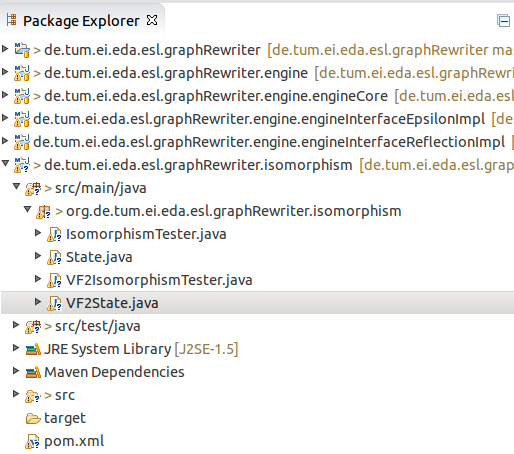
\includegraphics[width=0.6\columnwidth]{figures/folder.png}
}
\caption{folder structure}
\label{folder}
\end{figure}

Figure \ref{folder} shows the VF2 implementation in the current project.
As seen in the figure \ref{folder}
IsomorphismTester.java is an interface which defines a function which will be implemented in VF2IsomorphismTester.java.
\\
\\

\begin{lstlisting}[language = Java,frame = single]
public interface IsomorphismTester {
/*
 * Return true if the graphs are Isomorphic
 */
boolean areIsomorphic(Graph<EObject, EClass> g1, Graph<EObject, EClass> g2);
}
\end{lstlisting}

State.java is an interface, which corresponds to the state s of the VF2 algorithm. VF2State.java implements State interface. 
\\

Some of the data structures used are,

\begin{lstlisting}[language = Java,frame = single]
/*possible candidates to add it to state */
private ArrayList<Pair<EObject>> candidates; 
	
private ArrayList<EObject> sourcePath; // Holds matched vertices of source
private ArrayList<EObject> targetPath; // Holds matched vertices of target

\end{lstlisting}

VF2IsomorphismTester.java defines match procedure along with implementing areIsomorphic() function. 

\begin{lstlisting}[language = Java,frame = single]
private boolean match(State s) {
		if(s.isGoal()){
			maps.add(s.getVetexMapping());
			return true;
		}
		if(s.isDead())
			return false;
		
		boolean found = false;		
		while(!found && s.hasNextCandidate()){
			Pair<EObject> candidate = s.nextCandidate();
					
			if(s.isFeasiblePair(candidate)) {
				State nextState = s.nextState(candidate);
						
				found = match(nextState);
			
				if(nextState.backtrack()){			
				}
				else{
					return false;
				}
			}
	}
		return found;
}
\end{lstlisting}

s.isGoal() returns true if all vertices are mapped.\\
s.isDead() returns false when vertex number mismatch happens. 

After the necessary checks, it choses the initial candidate as our start node pair and checks for feasibility of the candidate. And if it is a feasible candidate, a next state is created, with the current candidate added to $map$.
And the match procedure is called on the next state. Once we run out of candidates, the match function returns and checks for backtracking. If it is a successful backtrack, the matching continues. Otherwise, match terminates by returning false. \\

\texttt{s.nextState():}
\texttt{s.nextState} returns a new VF2State by copying all the previous state values and adding the current candidate to the state. Additionally, it loads the new candidates for matching, which are the combinations of neighbors of previous candidates. 

\section{Results}
Most of the comparisons were eliminated by negative checks and the individual node matching step. For a graph having 315 nodes, the time taken for a successful match is 17 seconds and for an unsuccessful match is 12.5 seconds. This is a good result considering the setup time.

Figure \ref{result} shows the resulting graph obtained by node merge. 
\begin{figure}
 \centerline{
 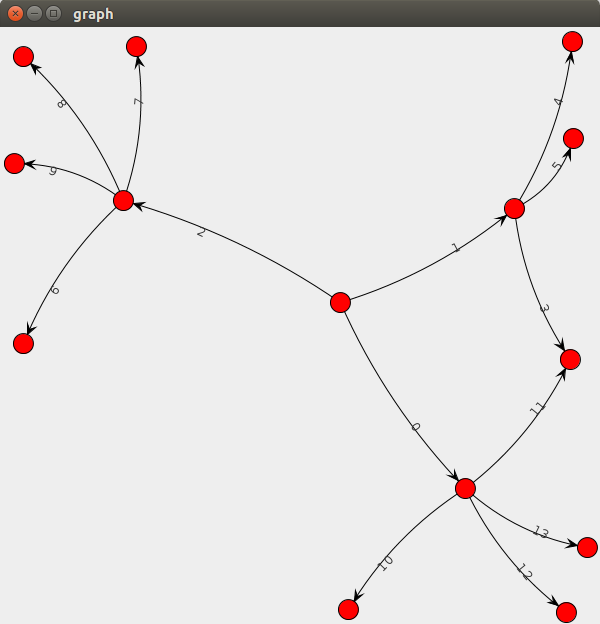
\includegraphics[width=1.0\columnwidth]{figures/result.png}
 }
 \caption{Resultant graph after node merge \cite{vf2}}
 \label{result}
 \end{figure}
 



\chapter{Other Work} \label{gmf}
This chapter explains the work carried out on grahical modeling framework and GrGen and the possibility of using them with current graph rewriting project.

\begin{figure}
 \centerline{
 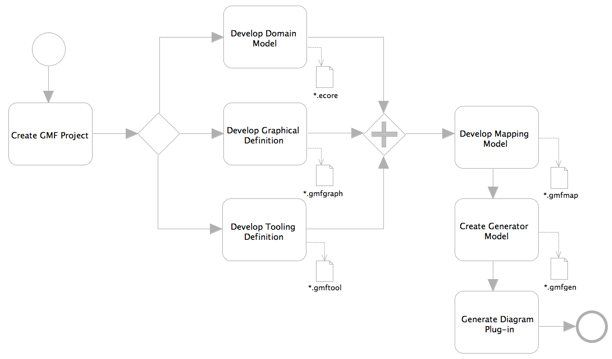
\includegraphics[width=1.0\columnwidth]{figures/gmf.png}
 }
 \caption{Overview of GMF}
 % Quote GMF website
 \label{gmf}
 \end{figure}

\section{Graphical Modeling Project}
The Eclipse Graphical Modeling Project (GMP) provides a set of generative components and runtime infrastructures for developing graphical editors based on EMF and GEF. Since the current graph is built on EMF, it is easy to extend the project to have a graphical editor based on GEF (Graphical Editing Framework). The Graphical Modeling Framework (GMF) Tooling project provides a model-driven approach to generating graphical editors in Eclipse \cite{gmf}.

The GMF runtime is an industry proven application framework for creating graphical editors using EMF and GEF. With these things in picture a graphical editor can be easily created 

\subsection{GMF-Tooling workflow}
The diagram \ref{gmf} illustrates the main components and the work flows of the GMF. 

Once creating the initial project the first task is to create a domain model or use an existing domain model(.ecore). Core to GMF is the concept of a graphical definition model. This model contains information related to the graphical elements that will appear in a GEF-based runtime. An optional tooling definition model is used to design the palette and other periphery (menus, toolbars, etc.). Once the appropriate mappings are defined, GMF provides a generator model to allow implementation details to be defined for the generation phase. The production of an editor plug-in based on the generator model will target a final model. GMF provides this work-flow in eclipse making it easy to generate. 


\section{GrGen}
GrGen (Graph Rewrite Generator) is a software development tool that offers programming
languages optimized for graph structured data, with declarative pattern matching and rewriting at their core, with support for imperative and object-oriented programming, and a bit of database-like query-result processing\cite{grgen}. 

The idea of was to use GrGen for graph transformation. For this requirement was to convert the current graph format(JUNG - Java Universal Network/Graph Framework) to the graph system (explained below) understood by GrGen.NET system and transform the graph and convert it back to JUNG. 

GrGen.NET is fast and efficient but it needs a lot of effort to understand and use it.

Graph is represented using a language called graph modelling language(.gm) and rules are defined in $rule language (.grg)$  with embedded sequences. This rules on the Host graph can be controlled by a Shell script written in GrShell language or  C-sharp application. These can be used for interactive debugging with the graph viewer. 

The central object is the graph, it adheres to the specified graph model. (In general
you have to distinguish between a graph model on the meta level, a host graph created as instance of the graph model, and a statically specified pattern graph of a rule that matches a portion of the host graph at runtime).\\

\begin{itemize}

\item {Reasons for consideration of GrGen.NET}
 
\begin{itemize}
\item GrGen.NET offers processing of graph representations at their natural level of abstraction. It is built on a rich and efficient metamodel implementing multi-graphs, with multiple inheritance on node and edge types. 

\item It reduces the graph transformation hassles(pointer modifications) which existed in low level languages.

\item GrGen.NET is one of the fastest available engines for graph transformation. 

\item Graphs can be exported to .XMI format. XMI files as written by the Eclipse Modeling Framework (EMF) are a standard format in the model transformation community.
\end{itemize}

\item{This project was discontinued because}
\begin{itemize}
\item Converting the graphs in to generic language is very complicated process. Since the idea was to convert any given JUNG graph to GrGen format. It is difficult to write a software that writes a another language. 

\item In the given time frame of the project it was not feasible to complete the work. 

\item The ROI (Return on Investment) was very less.  
\end{itemize}
\end{itemize}



\chapter{Conclusion}\label{chapter:conclusion}


\appendix{}

%\bibliographystyle{plain}
%\bibliography{bibliography/literature}{}
 % TODO: remove if glossary not needed
%\glsaddall{} % add all defined terms to glossary, even if not referenced in text
%\printglossaries{}

\microtypesetup{protrusion=false}
\listoffigures{}
%\listoftables{}
\microtypesetup{protrusion=true}
\printbibliography

\end{document}
